\section{The Derivative Function}\label{sec:TheDerivativeFunction}
In Section \ref{sec:Slope}, we have seen how to create, or derive, a new function $f'(x)$ from a
function $f(x)$, and that this new function carries important
information. In one example we saw that $f'(x)$ tells us how steep the
graph of $f(x)$ is; in another we saw that $f'(x)$ tells us the velocity
of an object if $f(x)$ tells us the  position of the object at time
$x$. As we said earlier, this same mathematical idea is useful
whenever $f(x)$ represents some changing quantity and we want to know
something about how it changes, or roughly, the ``rate'' at which it
changes. Most functions encountered in practice are built up from a
small collection of ``primitive'' functions in a few simple ways, for
example, by adding or multiplying functions together to get new, more
complicated functions. To make good use of the information provided by
$f'(x)$ we need to be able to compute it for a variety of such functions.

We will begin to use different notations for the derivative of a
function. While initially confusing, each is often useful so it is
worth maintaining multiple versions of the same thing.

Consider again the function $\ds f(x)=\sqrt{625-x^2}$.
We have computed the derivative $\ds f'(x)=-x/\sqrt{625-x^2}$, and have
already noted that if we use the alternate notation
$\ds y=\sqrt{625-x^2}$ then we might write $\ds y'=-x/\sqrt{625-x^2}$.
Another notation is quite different, and in time it will become clear
why it is often a useful one. Recall that to compute the the
derivative of $f$ we computed 
$$
\lim_{\Delta x\to0} {\sqrt{625-(7+\Delta x)^2} - 24\over \Delta x}.
$$
The denominator here measures a distance in the $x$ direction,
sometimes called the ``run'', and the numerator measures a distance in
the $y$ direction, sometimes called the ``rise,'' and ``rise over
run'' is the slope of a line. Recall that sometimes such a numerator is
abbreviated $\Delta y$, exchanging brevity for a more detailed
expression. So in general, we define a derivative by the following equation.

\begin{definition}{Defnition of Derivative}{DerDefn}
The derivative of $y=f(x)$ with respect to $x$ is
$$y'=\lim_{\Delta x\to0} {\Delta y\over \Delta x}.$$
Some textbooks use $h$ in place of $\Delta x$ in the definition of
derivative: $$f'(x)=\lim_{h\to 0}\frac{f(x+h)-f(x)}{h}.$$ 
\end{definition}

To recall the form of the limit, we sometimes say instead that
$$
{dy\over dx}=\lim_{\Delta x\to0} {\Delta y\over \Delta x}.
$$ 
In other words, $dy/dx$ is another notation for the derivative, and
it reminds us that it is related to an actual slope between two
points. This notation is called \dfont{Leibniz notation}, 
after Gottfried Leibniz, who developed the fundamentals
of calculus independently, at about the same time that Isaac Newton
did.  Again, since we often use $f$ and $f(x)$ to mean the original
function, we sometimes use $df/dx$ and $df(x)/dx$ to refer to the
derivative. If the function $f(x)$ is written out in full we often
write the last of these something like this
$$f'(x)={d\over dx}\sqrt{625-x^2}$$
with the function written to the side, instead of trying to fit it into
the numerator.

\begin{example}{Derivative of $y=t^2$}{Derivative1}
Find the derivative of $\ds y=f(t)=t^2$.
\end{example}

\begin{solution} 
We compute 
\[ \begin{array}{rll}
y' &=& \ds\lim_{\Delta t\to0}\ds\frac{\Delta y}{\Delta t}  \\
\\
	&=&\ds\lim_{\Delta t\to0}\ds\frac{(t+\Delta t)^2-t^2}{\Delta t} \\
	\\
&=&\ds\lim_{\Delta t\to0}\ds\frac{t^2+2t\Delta t+\Delta t^2-t^2}{\Delta t} \\
\\
&=&\ds\lim_{\Delta t\to0}\ds\frac{2t\Delta t+\Delta t^2}{\Delta t} \\
\\
&=&\ds\lim_{\Delta t\to0} 2t+\Delta t=2t. \\
\end{array}\]
\end{solution}

Remember that $\Delta t$ is a single quantity, not a ``$\Delta$''
times a ``$t$'', and so $\ds \Delta t^2$ is $\ds (\Delta t)^2$ not 
$\ds \Delta (t^2)$.
Doing the same example using the second formula for the derivative with $h$ in place of $\Delta t$ gives the following.
Note that we compute $f(t+h)$ by substituting $t+h$ in place of $t$ everywhere we see $t$ in the expression $f(t)$,
\textit{while making no other changes} (at least initially). For example, if $f(t)=t+\sqrt{(t+3)^2-t}$ then $f(t+h)=(t+h)+\sqrt{((t+h)+3)^2-(t+h)}=t+h+\sqrt{(t+h+3)^2-t-h}$.

\begin{example}{Derivative of $y=t^2$}{Derivative1b}
Find the derivative of $\ds y=f(t)=t^2$.
\end{example}

\begin{solution} 
We compute 
\[ \begin{array}{rll}
f'(t) &=& \ds\lim_{h\to0}\ds\frac{f(t+h)-f(t)}{h}  \\
\\
	&=&\ds\lim_{h\to0}\ds\frac{(t+h)^2-t^2}{h} \\
	\\
&=&\ds\lim_{h\to0}\ds\frac{t^2+2th+h^2-t^2}{h} \\
\\
&=&\ds\lim_{h\to0}\ds\frac{2th+h^2}{h} \\
\\
&=&\ds\lim_{h\to0} 2t+h=2t. \\
\end{array}\]
\end{solution}

\begin{example}{Derivative}{Derivative2}
Find the derivative of $y=f(x)=1/x$.
\end{example}

\begin{solution} 
The computation:
\begin{eqnarray*}
y' &=& \lim_{\Delta x\to0}{\Delta y\over\Delta x}\cr
\\
&=&\lim_{\Delta x\to0}{ {1\over x+\Delta x} - {1\over x}\over \Delta
  x}\cr
\\
&=&\lim_{\Delta x\to0}{ {x\over x(x+\Delta x)} - 
{x+\Delta x\over x(x+\Delta x)}\over \Delta x}\cr
\\
&=&\lim_{\Delta x\to0}{ {x-(x+\Delta x)\over x(x+\Delta x)}\over \Delta x}\cr
\\
&=&\lim_{\Delta x\to0} {x-x-\Delta x\over x(x+\Delta x)\Delta x}\cr
\\
&=&\lim_{\Delta x\to0} {-\Delta x\over x(x+\Delta x)\Delta x}\cr
\\
&=&\lim_{\Delta x\to0} {-1\over x(x+\Delta x)}={-1\over x^2}\cr
\end{eqnarray*}
\end{solution}

{\bf Note:}  If you happen to know some ``derivative formulas'' from
an earlier course, for the time being you should pretend that you do
not know them.
In examples like the ones above and the exercises below, you are required
to know how to find the derivative formula starting from basic principles.
We will later develop some formulas so that we do not always need to
do such computations, but we will continue to need to know how to do
the more involved computations.

To recap, given any function $f$ and any number $x$ in the domain of $f$, we define
$f'(x)=\lim_{h\to 0}\frac{f(x+h)-f(x)}{h}$ wherever this limit exists, and we call
the number $f'(x)$ the derivative of $f$ at $x$. Geometrically, $f'(x)$ is the slope of
the tangent line to the graph of $f$ at the point $(x,f(x))$.  The following
symbols also represent the derivative:
$$f'(x)=y'=\frac{dy}{dx}=\frac{df}{dx}=\frac{d}{dx}f(x).$$ The symbol
$d/dx$ is called a differential operator which means to take the
derivative of the function $f(x)$ with respect to the variable $x$.

In the next example we emphasize the geometrical interpretation of derivative.

\begin{example}{Geometrical Interpretation of Derivative}{GeometricalInterpretationDerivative}
Consider the function $f(x)$ given by the graph below.
Verify that the graph of $f'(x)$ is indeed the derivative of $f(x)$ by analyzing slopes of tangent lines to the graph at different points.
$$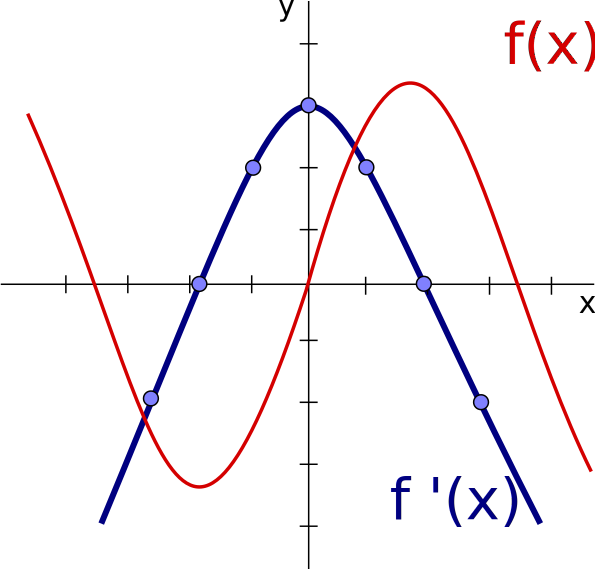
\includegraphics[width=2.5in]{images/deriv1}$$
\end{example}

\begin{solution} 
We must think about the tangent lines to the graph of $f$, because the slopes
of these lines are the values of $f'(x)$.

We start by checking the graph of $f$ for horizontal tangent lines, since horizontal
lines have a slope of 0. We find that the tangent line is horizontal at the points
where $x$ has the values -1.9 and 1.8 (approximately). At each of these values of $x$,
we must have $f'(x)=0$, which means that the graph of $f'$ has an $x$-intercept (a point
where the graph intersects the $x$-axis). 

Note that horizontal tangent lines have a slope of zero and these
occur approximately at the points $(-1.9,-3.2)$ and $(1.8,3.2)$ of the
graph.  Therefore $f'(x)$ will cross the $x$-axis when $x=-1.9$ and
$x=1.8$.  

Analyzing the slope of the tangent line of $f(x)$ at $x=0$ gives
approximately $3.0$, thus, $f'(0)=3.0$.  Similarly, analyzing the
slope of the tangent lines of $f(x)$ at $x=1$ and $x=-1$ give
approximately $2.0$ for both, thus, $f'(1)=f'(-1)=2.0$.
\end{solution}

In the next example we verify that the slope of a straight line is $m$.

\begin{example}{Derivative of a Linear Function}{DerivativeLinearFunction}
Let $m,b$ be any two real numbers.
Determine $f'(x)$ if $f(x)=mx+b$.
\end{example}

\begin{solution} 
By the definition of derivative (using $h$ in place of $\Delta x$) we have,
$$f'(x)=\lim_{h\to 0}\frac{f(x+h)-f(x)}{h}=\lim_{h\to 0}\frac{(m(x+h)+b)-(mx+b)}{h}$$
$$=\lim_{h\to 0}\frac{mh}{h}=\lim_{h\to 0}m=m.$$

This is not surprising. We know that $f'(x)$ always represents the slope of a tangent
line to the graph of $f$. In this example, since the graph of $f$ is a straight line $y=mx+b$
already, every tangent line is the same line $y=mx+b$. Since this line has a slope of $m$,
we must have $f'(x)=m$.
\end{solution}

%%%%%%%%%%%%%%%%%%%%%%%%%%%%%%%%%%%%%%%%%%%%%%%%%
% Subsections to include
%%%%%%%%%%%%%%%%%%%%%%%%%%%%%%%%%%%%%%%%%%%%%%%%%
\subsection{Differentiable}
Now that we have introduced the derivative
of a function at a point, we can begin to use the adjective \dfont{differentiable}.

\begin{definition}{Differentiable at a Point}{DifferentiablePoint}
A function $f$ is
differentiable at point $a$ if $f'(a)$ exists.
\end{definition}

\begin{definition}{Differentiable on an Interval}{Differentiable}
A function $f$ is differentiable on an open interval if it is differentiable at every point in the interval.
\end{definition}

Sometimes one encounters a point in the domain of a function $y=f(x)$ where
there is {\bf no derivative}, because there is no tangent line.  In order
for the notion of the tangent line at a point to make sense, the curve must
be ``smooth'' at that point.  This means that if you imagine a particle
traveling at some steady speed along the curve, then the particle does not
experience an abrupt change of direction.  There are two types of
situations you should be aware of---corners and cusps---where there's a
sudden change of direction and hence no derivative.

\begin{example}{Derivative of the Absolute Value}{DerivativeAbsoluteValue}
Discuss the derivative of the absolute value function $y=f(x)=|x|$.
\end{example}

\begin{solution} 
If $x$ is positive, then this is the function $y=x$, whose derivative is
the constant 1.  (Recall that when $y=f(x)=mx+b$, the derivative is the
slope $m$.)  If $x$ is negative, then we're dealing with the function $y=-x$,
whose derivative is the constant $-1$.  If $x=0$, then the function has
a corner, i.e., there is no tangent line.  A tangent line 
would have to point in the direction of the curve---but there are {\it
two} directions of the curve that come together at the origin.

$$\includegraphics[width=2.5in]{images/absvalue}$$

We can summarize this as
$$ 
y'=\left\{\begin{array}{rl}
1, & \mbox{if $x>0$,}\\
-1, & \mbox{if $x<0$,}\\
\hbox{undefined,} & \mbox{if $x=0$.}\\
\end{array}\right.
$$
In particular, the absolute value function $f(x)=|x|$ is \ifont{not} differentiable at $x=0$.
\end{solution}

We note that the following theorem can be proved using limits.

\begin{theorem}{Differentiable implies Continuity}{DifferentiableImpliesContinuity}
If $f$ is differentiable at $a$, then $f$ is continuous at $a$.
\end{theorem}
\begin{proof}
Suppose that $f$ is differentiable at $a.$ That is,%
\begin{equation*}
	f^{\prime }\left( a\right) =\lim_{h\rightarrow 0}\frac{f\left( a+h\right)
		-f\left( a\right) }{h}
\end{equation*}%
exists. At this stage, we find it convenient to write this limit in an
alternative form so that its connection with continuity can become more
easily seen. If we let $x=a+h,$ then $h=x-a.$ Furthermore, $h\rightarrow 0$
is equivalent to $x\rightarrow a.$ So,%
\begin{equation*}
	f^{\prime }\left( a\right) =\lim_{x\rightarrow a}\frac{f\left( x\right)
		-f\left( a\right) }{x-a}.
\end{equation*}%
(This alternative formulation of the derivative is also standard. We will
use it whenever we find it convenient to do so. You should get familiar with
it.) Continuity at $a$ can now be proved as follows:%
\begin{eqnarray*}
	\lim_{x\rightarrow a}f\left( x\right) &=&\lim_{x\rightarrow a}\left( \frac{%
		f\left( x\right) -f\left( a\right) }{x-a}\cdot \left( x-a\right) +f\left(
	a\right) \right) \\
	&=&\lim_{x\rightarrow a}\frac{f\left( x\right) -f\left( a\right) }{x-a}\cdot
	\lim_{x\rightarrow a}\left( x-a\right) +\lim_{x\rightarrow a}f\left( a\right)
	\\
	&=&f^{\prime }\left( a\right) \cdot \left( a-a\right) +f\left( a\right) \\
	&=&f\left( a\right).
\end{eqnarray*}
\end{proof}

However, if $f$ is continuous at $a$ it is \ifont{not} necessarily
true that $f$ is differentiable at $a$.  For example, it was shown
that $f(x)=|x|$ is not differentiable at $x=0$ in the previous
example, however, one can observe that $f(x)=|x|$ is continuous
everywhere.

\begin{example}{Derivative of $\ds y=x^{2/3}$}{Derivative}
Discuss the derivative of the function $\ds y=x^{2/3}$, shown in
Figure~\ref{fig:cusp}. 
\end{example}

\begin{solution} 
We will later see how to compute this
derivative; for now we use the fact that $\ds
y'=(2/3)x^{-1/3}$. Visually this looks much like the absolute value
function, but it technically has a cusp, not a corner. The absolute
value function has no tangent line at 0 because there are (at least)
two obvious contenders---the tangent line of the left side of the
curve and the tangent line of the right side.
The function $\ds y=x^{2/3}$ does not have a tangent line at 0, but
unlike the absolute value function it can be said to have a single
direction: as we approach 0 from either side the tangent line becomes
closer and closer to a vertical line; the curve is vertical at 0. But
as before, if you imagine traveling along the curve, an abrupt change
in direction is required at 0: a full 180 degree turn.  
\end{solution}

\figure
\centerline{\vbox{\beginpicture
\normalgraphs
%\ninepoint
\setcoordinatesystem units <2truecm,2truecm>
\setplotarea x from -2 to 2, y from 0 to 1.6
\axis left shiftedto x=0 ticks numbered from 0 to 1 by 1 /
\axis bottom ticks numbered from -2 to 2 by 1 /
\setquadratic
\plot -2.000 1.587 -1.933 1.552 -1.867 1.516 -1.800 1.480 -1.733 1.443 
-1.667 1.406 -1.600 1.368 -1.533 1.330 -1.467 1.291 -1.400 1.251 
-1.333 1.211 -1.267 1.171 -1.200 1.129 -1.133 1.087 -1.067 1.044 
-1.000 1.000 -0.933 0.955 -0.867 0.909 -0.800 0.862 -0.733 0.813 
-0.667 0.763 -0.600 0.711 -0.533 0.658 -0.467 0.602 -0.400 0.543 
-0.333 0.481 -0.267 0.414 -0.200 0.342 -0.133 0.261 -0.067 0.164 
0.000 0.000 0.067 0.164 0.133 0.261 0.200 0.342 0.267 0.414 
0.333 0.481 0.400 0.543 0.467 0.602 0.533 0.658 0.600 0.711 
0.667 0.763 0.733 0.813 0.800 0.862 0.867 0.909 0.933 0.955 
1.000 1.000 1.067 1.044 1.133 1.087 1.200 1.129 1.267 1.171 
1.333 1.211 1.400 1.251 1.467 1.291 1.533 1.330 1.600 1.368 
1.667 1.406 1.733 1.443 1.800 1.480 1.867 1.516 1.933 1.552 
2.000 1.587   /
\endpicture}}
\caption{A cusp on $\ds x^{2/3}$. \label{fig:cusp}}
\endfigure

In practice we won't worry much about the distinction between these
examples; in both cases the function has a ``sharp point'' where there
is no tangent line and no derivative.
\subsection{Second and Other Derivatives}
If $f$ is a differentiable function then its derivative $f'$ is also a function and so we can take the derivative of $f'$.
The new function, denoted by $f''$, is called the \dfont{second derivative} of $f$, since it is the derivative of the derivative of $f$.

The following symbols represent the second derivative:
$$f''(x)=y''=\frac{d^2y}{dx^2}=\frac{d}{dx}\left(\frac{dy}{dx}\right).$$

We can continue this process to get the third derivative of $f$.

In general, the \dfont{$n$th derivative} of $f$ is denoted by $f^{(n)}$ and is obtained from $f$ by differentiating $n$ times.
If $y=f(x)$, then we write:
$$y^{(n)}=f^{(n)}(x)=\frac{d^ny}{dx^n}.$$
\subsection{Velocities}
Suppose $f(t)$ is a position function of an object, representing the displacement of the object from the origin at time $t$.
In terms of derivatives, the \dfont{velocity of an object is:}
$$v(a)=f'(a)$$
The change of velocity with respect to time is called the \dfont{acceleration} and can be found as follows:
$$a(t)=v'(t)=f''(t).$$
Acceleration is the derivative of the velocity function and the second derivative of the position function.

\begin{example}{Position, Velocity and Acceleration}{PositionFunction}
Suppose the position function of an object is $f(t)=t^2~metres$ at $t$ seconds.
Find the velocity and acceleration of the object at time $t=1s$.
\end{example}

\begin{solution} 
By the definition of velocity and acceleration we need to compute $f'(t)$ and $f''(t)$.
Using the definition of derivative, we have,
$$f'(t)=\lim_{h\to 0}\frac{(t+h)^2-t^2}{h}=\lim_{h\to 0}\frac{2th+h^2}{h}=\lim_{h\to 0}(2t+h)=2t.$$
Therefore, $v(t)=f'(t)=2t$.
Thus, the velocity at time $t=1$ is $v(1)=2~m/s$.
We now have that the acceleration at time $t$ is:
$$a(t)=f''(t)=\lim_{h\to 0}\frac{2(t+h)-2t}{h}=\lim_{h\to 0}\frac{2h}{h}=2.$$
Therefore, $a(t)=2$.
Substituting $t=1$ into the function $a(t)$ gives $a(1)=2~m/s^2$.
\end{solution}



%%%%%%%%%%%%%%%%%%%%%%%%%%%%%%%%%%%%%%%%%%%%%%%%%
\Opensolutionfile{solutions}[ex]
\section*{Exercises for Section \ref{sec:TheDerivativeFunction}}

\begin{enumialphparenastyle}

%%%%%%%%%%
\begin{ex} 
Find the derivatives of the following functions.
\begin{enumerate}
	\item	$\ds y=f(x)=\sqrt{169-x^2}$
	\item	$\ds y=f(t)=80-4.9t^2$
	\item	$\ds y=f(x)=x^2-(1/x)$
	\item	$\ds y=f(x)=ax^2+bx+c$, where $a$, $b$, and $c$ are constants.
	\item	$\ds y=f(x)=x^3$
	\item	$\ds y=f(x)=2/\sqrt{2x+1}$
	\item	$y=g(t)=(2t-1)/(t+2)$
\end{enumerate}
\begin{sol}
\begin{enumerate}
	\item	$\ds -x/\sqrt{169-x^2}$
	\item	$-9.8t$
	\item	$\ds 2x+1/x^2$
	\item	$2ax+b$
	\item	$\ds 3x^2$
	\item	$\ds -2/(2x+1)^{3/2}$
	\item	$\ds 5/(t+2)^2$
\end{enumerate}
\end{sol}
\end{ex}

%%%%%%%%%%
\begin{ex} 
Shown is the graph of a function $f(x)$. Sketch the graph of $f'(x)$
by estimating the derivative at a number of points in the interval:
estimate the derivative at regular intervals from one end of the
interval to the other, and also at ``special'' points, as when the
derivative is zero. Make sure you indicate any places where the
derivative does not exist.
$$\vbox{\beginpicture
\normalgraphs
\setcoordinatesystem units <4.5truecm,4.5truecm>
\setplotarea x from -1 to 1, y from 0 to 1.6
\axis left ticks numbered from 0.2 to 1.6 by 0.2 /
\axis left shiftedto x=0 /
\axis bottom ticks numbered from -1 to 1 by 0.2 /
\setquadratic
\plot -0.900 0.800 -0.810 1.003 -0.720 1.148 -0.630 1.242 -0.540 1.291 
-0.450 1.301 -0.360 1.280 -0.270 1.232 -0.180 1.166 -0.090 1.086 
0.000 1.000 0.090 0.914 0.180 0.834 0.270 0.768 0.360 0.720 
0.450 0.699 0.540 0.709 0.630 0.758 0.720 0.852 0.810 0.997 
0.900 1.200  /
\linethickness 0.1truept
\axis left ticks in andacross from 0.1 to 1.6 by 0.1 /
\axis bottom ticks in andacross from -1 to 1 by 0.1 /
\endpicture}$$
\end{ex}

%%%%%%%%%%
\begin{ex} 
Shown is the graph of a function $f(x)$. Sketch the graph of $f'(x)$
by estimating the derivative at a number of points in the interval:
estimate the derivative at regular intervals from one end of the
interval to the other, and also at ``special'' points, as when the
derivative is zero. Make sure you indicate any places where the
derivative does not exist.
$$\vbox{\beginpicture
\normalgraphs
\setcoordinatesystem units <1.8truecm,1.8truecm>
\setplotarea x from 0 to 5, y from 0 to 4
\axis left ticks numbered from 0 to 4 by 1 /
\axis bottom ticks numbered from 0 to 5 by 1 /
\plot 0 0 2 2 /
\setquadratic
\plot 2.000 2.000 2.135 1.747 2.270 1.531 2.405 1.351 2.540 1.209 
2.675 1.103 2.810 1.034 2.945 1.002 3.080 1.007 3.215 1.049 
3.350 1.128 3.485 1.244 3.620 1.396 3.755 1.586 3.890 1.812 
4.025 2.075 4.160 2.375 4.295 2.712 4.430 3.086 4.565 3.497 
4.700 3.945  /
\linethickness 0.1truept
\axis left ticks in andacross from 0.2 to 4 by 0.2 /
\axis bottom ticks in andacross from 0.2 to 5 by 0.2 /
\endpicture}$$
\end{ex}

%%%%%%%%%%
\begin{ex} 
Find an equation for the tangent line to the graph of $\ds f(x)=5-x-3x^2$ at the point $x=2$
\begin{sol}
	$y=-13x+17$
\end{sol}
\end{ex}

%%%%%%%%%%
\begin{ex} 
Find a value for $a$ so that the graph of $\ds f(x)=x^2+ax-3$ has a horizontal tangent line at $x=4$.
\begin{sol}
	$-8$
\end{sol}
\end{ex}

\end{enumialphparenastyle}